




\begin{table*}
\begin{center}

 \textbf{Conceptual Captions}
\begin{tabular}{lccccc}
\toprule
Model &  ROUGE-L  & CIDEr  & SPICE  & \#Params (M)  & Training Time   \\ 
\bottomrule
\midrule
VLP &  &  &  & 115 & h (V)\\
\toprule
Ours; MLP + GPT2 tuning &  &  &  &  & h (GTX)\\
\midrule
Ours; Transformer &  &  &  &  & \textbf{h} (GTX) \\
\bottomrule 
\end{tabular}
\vspace{0.15cm}

 \textbf{nocaps}


\begin{tabular}{p{0.17\textwidth}|cc|cc|cc|cc|cc}
\toprule

& \multicolumn{2}{c}{in-domain} & \multicolumn{2}{c}{near-domain} & \multicolumn{2}{c}{out-of-domain} & \multicolumn{2}{c}{Overall} & & \\
Model &  CIDEr   & SPICE   & CIDEr & SPICE & CIDEr & SPICE & CIDEr & SPICE & Params & Time  \\ 
\bottomrule
\midrule
BUTD ~\cite{anderson2018bottom}  &  &  &  &  &  &  &  &  &  & h  \\
\midrule
Oscar ~\cite{li2020oscar} &  &  &  &  &  &  &  &  &  & h\\
\toprule
Ours; MLP + GPT2 tuning &  &  &  &  &  &  &  & &  & h\\
\midrule
Ours; Transformer &  &  &  &  &  &  &  &  & & \textbf{h} \\
\midrule
\end{tabular}

\vspace{0.15cm}
 \textbf{COCO}


\begin{tabular}{p{0.26\textwidth}cccccc}
\toprule
Model &   B@  & METEOR  & CIDEr  & SPICE  & \#Params (M)  & Training Time  \\ 
\bottomrule
\midrule
BUTD ~\cite{anderson2018bottom} &   &  &  &  & 52 & h (M)\\
\midrule
VLP ~\cite{zhou2020unified} &   &  &  &  & 115 & h (V)\\
\midrule
Oscar ~\cite{li2020oscar} &  &  &   &  &   & h (V)\\

\toprule
Ours; Transformer   &  &  &   &  &  & \textbf{h} (GTX)\\
\midrule

Ours; MLP + GPT2 tuning &  &  &   &  &  & h (GTX)\\

\midrule

\multicolumn{7}{c}{ \textbf{Ablation}} \\
\bottomrule
\midrule

Ours; Transformer + GPT2 tuning  &  &  &   &  &  & h (GTX) \\

\midrule
Ours; MLP &  &  &  &  &  & h (GTX)\\
\midrule

\end{tabular}


\end{center}
\vspace{-0.1cm}
\caption{Quantitative evaluation. As can be seen, our method achieves comparable results for both nocaps and Conceptual Captions with much faster training time. }
\label{tab:num} 
\end{table*} 
























\begin{figure*}
\footnotesize
\centering
\begin{tabular}{p{0.2\columnwidth} p{0.33\columnwidth}p{0.33\columnwidth}p{0.33\columnwidth}p{0.33\columnwidth}p{0.32\columnwidth}}
&
\includegraphics[trim={2cm 0 0 0},clip,width=0.34\columnwidth,height=0.22\columnwidth]{images/COCO_val2014_000000391895.jpg} &
\includegraphics[width=0.34\columnwidth,height=0.22\columnwidth]{images/COCO_val2014_000000060623.jpg} &
\includegraphics[trim={0, .1cm 0 .2cm},clip,width=0.34\columnwidth,height=0.22\columnwidth]{images/COCO_val2014_000000483108_crop.jpg} &
\includegraphics[trim={0 10cm 0 2cm},clip,width=0.34\columnwidth,height=0.22\columnwidth]{images/COCO_val2014_000000386164.jpg} &
\includegraphics[trim={0 1cm 0 1cm},clip,width=0.34\columnwidth,height=0.22\columnwidth]{images/COCO_val2014_000000384213.jpg} \\
\begin{tabular}{l}Ground Truth \end{tabular}& A man with a red helmet on a small moped on a dirt road & A young girl inhales with the intent of blowing out a candle.  
& A man on a bicycle riding next to a train. & a wooden cutting board topped with sliced up food.  & A kitchen is shown with a variety of items on the counters.\\
\hline
\begin{tabular}{l}Oscar \end{tabular}& a man riding a motorcycle down a dirt road. & a woman sitting at a table with a plate of food.  & a woman riding a bike down a street next to a train. & a woman sitting at a table with a plate of food.  & a kitchen with a sink, dishwasher and a window.\\
\hline
\begin{tabular}{l}
Ours; MLP + \\ GPT2 tuning
\end{tabular}& a man riding a motorcycle on a dirt road. & a woman is eating a piece of cake with a candle. & a man is standing next to a train. & a row of wooden cutting boards with wooden spoons. & a kitchen with a sink, stove, and window.\\
\hline
\begin{tabular}{l}
Ours; \\ Transformer
\end{tabular}  & a man is riding a motorbike on a dirt road. & a young girl sitting at a table with a cup of cake. &  a man is standing next to a train.  & a wooden table with a bunch of wood tools on it.   & a kitchen with a sink and a window. \\

\end{tabular}
\vspace{-0.2cm}
\caption{Uncurated results of the first five images in the COCO test set (Karpathy et al.~\cite{karpathy2015deep} split).}\vspace{-0.2cm}
\label{fig:img} 
\end{figure*} 





















\begin{figure*}
\footnotesize
\centering
\begin{tabular}{p{0.2\columnwidth} p{0.33\columnwidth}p{0.33\columnwidth}p{0.33\columnwidth}p{0.33\columnwidth}p{0.33\columnwidth}}
&
\includegraphics[trim={0 3cm 0 2cm},clip,width=0.34\columnwidth,height=0.24\columnwidth]{images/00.jpg} &
\includegraphics[trim={0 2cm 0 0},clip,width=0.34\columnwidth,height=0.24\columnwidth]{images/01_crop.jpg} &
\includegraphics[trim={0 .1cm 0 .2cm},clip,width=0.34\columnwidth,height=0.24\columnwidth]{images/03_crop.jpg} &
\includegraphics[width=0.34\columnwidth,height=0.24\columnwidth]{images/02.jpg} &
\includegraphics[width=0.34\columnwidth,height=0.24\columnwidth]{images/04.jpg} \\

\begin{tabular}{l}Ground Truth \end{tabular}& A life in photography -- in pictures. & Photograph of the sign being repaired by brave person. 
& Globes : the green 3d person carrying in hands globe. &  The player staring intently at a computer screen.  & The - bedroom stone cottage can sleep people.\\
\hline
\begin{tabular}{l}VLP \end{tabular}&  Actors in a scene from the movie. & The sign at the entrance.  & Templates: green cartoon character holding the earth globe. & Person works on a video.  &  The master bedroom has a king - sized bed with a queen size bed.  \\
\hline
\begin{tabular}{l}
Ours; MLP +\\ GPT2 tuning
\end{tabular}& Actor sits in a hotel room. & The sign at the entrance. & 3d render of a man holding a globe. & Person, a student, watches a video on his laptop.  & The property is on the market for £ 1.\\
\hline
\begin{tabular}{l}
Ours; \\ Transformer
\end{tabular}& person sitting on a chair in a room. & a sign is seen at the entrance to the store. & stock image of a man holding the earth. & portrait of a young boy playing video game. & one of the bedrooms in the house has been converted into a living room. 


\end{tabular}
\caption{ Uncurated results of the first five images in our test set for Conceptual Captions \cite{sharma2018conceptual}.}
\label{fig:img_conceptual} 
\end{figure*}
 \begin{figure}
  \centering
  \footnotesize

\renewcommand{\arraystretch}{1}
\setlength{\tabcolsep}{3pt}

  \centering
  \footnotesize
\begin{tabular}{p{\imagew} p{\imagew} p{\imagew}  p{\imagew}}


\includegraphics[width=0.4\columnwidth,height=0.25\columnwidth]{images/IMG_2039.jpg} &
\includegraphics[width=0.4\columnwidth,height=0.25\columnwidth]{images/IMG_3461_2.jpg} \\
A person standing in front of a rock formation in the desert. & A man holding a banana in front of a river. \\
\\
\includegraphics[width=0.4\columnwidth,height=0.25\columnwidth]{images/IMG_1900.jpg} &
\includegraphics[width=0.4\columnwidth,height=0.25\columnwidth]{images/IMG_0277.jpg} \\
Two horned goats crossing a road in the desert. & A person sitting at a table with a tray of sushi. \\
 
\end{tabular}
\caption{Results over smartphone photos. Top: using our Conceptual Captions model. Bottom: COCO model. As demonstrated, our approach generalizes well to newly photographed images.}
\label{fig:real} 
\end{figure}



 

\section{Results}
\label{sec:res} 

\paragraph{Datasets.}

We use the \textit{COCO-captions} \cite{lin2014microsoft, chen2015microsoft}, \textit{nocaps} \cite{agrawal2019nocaps} , and \textit{Conceptual Captions} \cite{sharma2018conceptual} datasets. We split the former according to the Karpathy et al.~\cite{karpathy2015deep} split, where the training set contains  images and  captions per image. Since COCO is limited to  classes, the nocaps dataset is designed to measure generalization to unseen classes and concepts. It contains only validation and test sets, with the training utilizing COCO itself. The nocaps dataset is divided to three parts --- \textit{in-domain} contains images portraying only COCO classes, \textit{near-domain} contains both COCO and novel classes, and \textit{out-of-domain} consists of only novel classes. As suggested by Li et al.~\cite{li2020oscar}, we evaluate the model using only the validation set. Though some methods utilize object tags of the novel classes, we only consider the setting of no additional supervision, as we find it more applicable in practice. Therefore, we do not employ a constrained beam search \cite{anderson2016guided}.
The Conceptual Captions dataset consists of M pairs of images and captions, harvested from the web and post-processed. It is considered to be more challenging than COCO due to the larger variety of styles of both the images and the captions, while not limited to specific classes. To focus on the concepts, specific entities in this dataset are replaced with general notions. For example, in Fig.~\ref{fig:teaser}, the names are replaced with "politician". For evaluation, we use the validation set, consisting of K images, as the test set is not publicly available. Consequently, we did not use this set for validation. 





\paragraph{Baselines.}
We compare our method to the state-of-the-art works of Li et al.~\cite{li2020oscar} (known as Oscar), Vision-Language Pre-training model (VLP) \cite{zhou2020unified}, and the eminent work of Anderson et al.~\cite{anderson2018bottom}, denoted BUTD. 
These models first produce visual features using an object detection network \cite{ren2015faster}. BUTD then utilizes an LSTM to generate the captions, while VLP and Oscar employ a transformer, trained similarly to BERT \cite{devlin2018bert}. Both VLP and Oscar exploit an extensive pre-trained procedure over millions of image-text pairs.
Oscar \cite{li2020oscar} also uses additional supervision compared to our setting, in the form of object tags for each image.


Our default configuration employs the transformer mapping network, without fine-tuning the language model, denoted \textbf{Ours; Transformer}. Additionally, we also evaluate our variant that utilizes the MLP mapping network, and fine-tunes the language model, denoted \textbf{Ours; MLP + GPT2 tuning}. Other configurations are evaluated in Tab.~\ref{tab:num}.


\paragraph{Evaluation metrics.}
Similar to Li et al.~\cite{li2020oscar}, we validate our results over the COCO dataset using the common metrics BLEU \cite{papineni2002bleu}, METEOR \cite{denkowski2014meteor},  CIDEr \cite{vedantam2015cider} and SPICE \cite{anderson2016spice}, and for the nocaps dataset using CIDEr and SPICE. For the Conceptual Captions, we report the ROUGE-L \cite{lin2004automatic}, CIDEr, and SPICE, as suggested by the authors \cite{sharma2018conceptual}. 


Furthermore, we measure the training time and the number of trainable parameters to validate the applicability of our method.
Reducing the training time allows to quickly obtain a new model for new data, create an ensemble of models, and decrease energy consumption. Similar to other works, we report training time in GPU hours, and the GPU model used. The number of trainable parameters is a popular measure to indicate model feasibility. 














\begin{figure*}
\footnotesize
\centering
\begin{tabular}{l @{\hskip 5\tabcolsep} p{0.12\columnwidth}  p{0.35\columnwidth}p{0.35\columnwidth}p{0.35\columnwidth}p{0.35\columnwidth}p{0.35\columnwidth}}
& &
\includegraphics[width=0.36\columnwidth,height=0.27\columnwidth]{images/prefix_example-01.png} &
\includegraphics[width=0.36\columnwidth,height=0.27\columnwidth]{images/prefix_example-02.png} &
\includegraphics[trim={2cm 0cm 1cm 0cm},clip,width=0.36\columnwidth,height=0.27\columnwidth]{images/prefix_example-07.jpg} &
\includegraphics[width=0.36\columnwidth,height=0.27\columnwidth]{images/prefix_example-04.png} &
\includegraphics[width=0.36\columnwidth,height=0.27\columnwidth]{images/prefix_example-08.jpg} 
\\
\parbox[t]{0mm}{\multirow{2}{*}{\rotatebox[origin=c]{90}{\textbf{GPT- tuning}}}}
& Caption & a motorcycle is on display in a showroom. & a group of people sitting around a table. & a living room filled with furniture and a book shelf filled with books. & a fire hydrant is in the middle of a street. & display case filled with lots of different types of donuts. \\
& Prefix & com showcase motorcycle A ray motorcycleposed what polished Ink & blond vegetarian dishes dining expects smiling friendships group almost & tt sofa gest chair Bart books modern doorway bedroom & neon street Da alley putistan colorful nighttime & glass bakery dough displays sandwiches2 boxes Prin ten \\

\hline
\parbox[t]{0mm}{\multirow{2}{*}{\rotatebox[origin=c]{90}{\textbf{w/o tuning }}}}
& Caption & motorcycle that is on display at a show. & a a group of people sitting at a table together. & a living room with a couch and bookshelves. & a fire hydrant in front of a city street. & a display case full of different types of doughnuts.
\\
& Prefix & oover eleph SniperÃÂÃÂ motorcycle synergy undeniably achieving\textbackslash n & amic Delicious eleph SukActionCode photographers interchangeable undeniably achieving & orianclassic eleph CameroonÃÂÃÃÂroom synergy strikingly achieving\textbackslash n & ockets Pier eleph SniperÃÂÃÂ bicycl synergy undeniably achieving\textbackslash n & peanuts desserts elephbmÃÂÃÂÃ cooking nodd strikingly achieving\textbackslash n \\


\end{tabular}
\caption{Prefix Interpretability. We present both the generated caption and our prefix interpretation. Upper: Ours; MLP + GPT2 tuning. Bottom: Ours; Transformer.}
\label{fig:interpretation} 
\end{figure*}




 

\paragraph{Quantitative evaluation.}


Quantitative results for the challenging Conceptual Captions dataset are presented in Tab.~\ref{tab:num}.
As can be seen, we surpass the results of VLP, while requiring orders of magnitude less training time. We note that our lightweight model, which does not fine-tune GPT-, achieves an inferior result for this dataset. We hypothesize that due to the large variety of styles, a more expressive model is required than our light model, which induces a significantly lower parameter count. We compare only to VLP, as the other baselines haven't published results nor trained models for this dataset.



Tab.~\ref{tab:num} presents results for the nocaps dataset, where we achieve comparable results to the state-of-the-art method Oscar. As can be seen, 
Oscar achieves a slightly better SPICE score and we attain a slightly better CIDEr score. Still, our method uses a fraction of training time and trainable parameters with no additional object tags required, hence it is much more useful in practice. 


Tab.~\ref{tab:num} present the results for the COCO dataset. Oscar reaches the best results, however, it uses additional input in the form of object tags. Our results are closed to VLP and BUTD which utilize considerably more parameters and training time. Note that the training time of VLP and Oscar does not include the pre-training step. For instance, pre-training of VLP requires training over Conceptual Captions which consumes  GPU hours. 




Both Conceptual Captions and nocaps are designed to model a larger variety of visual concepts than COCO. Therefore, we conclude our method is preferable for generalizing to diverse data using a quick training procedure. This originates from utilizing the already rich semantic representations of both CLIP and GPT-.





\paragraph{Qualitative evaluation.}

Visual results of the uncurated first examples in our test sets of both Conceptual Captions and COCO datasets are presented in Figs.~\ref{fig:img} and \ref{fig:img_conceptual} respectively. As can be seen, our generated captions are meaningful and depict the image successfully for both datasets. We present additional examples collected from the web in Fig.~\ref{fig:teaser}. As can be seen, our Conceptual Captions model generalizes well to arbitrary unseen images as it was trained over a sizable and diverse set of images. We also present in Fig.~\ref{fig:real} results over smartphone images,  to further demonstrate generalization to new scenarios. Moreover, our model successfully identifies uncommon objects even when trained only over COCO. For example, our method recognizes the wooden spoons or the cake with a candle better than Oscar in Fig.~\ref{fig:img}, since CLIP is pre-trained over a diverse set of images. 
However, our method still fails in some cases, such as recognizing the bicycle next to the train in Fig.~\ref{fig:img}. This is inherited from the CLIP model, which does not perceive the bicycle in the first place. We conclude that our model would benefit from improving CLIP object detection ability, but leave this direction for future work.  
For Conceptual Captions, our method mostly produces accurate captions, such as perceiving the green d person in Fig.~\ref{fig:img_conceptual}. As expected, our method still suffers from data bias. For instance, it depicts the bedroom image in Fig.~\ref{fig:img_conceptual} as "The property is on the market for £ 1" after witnessing such captions of property advertising during training. 



\paragraph{Language model fine-tuning.}
As described in Section.~\ref{sec:method}, fine-tuning the language model results in a much more expressive model, but that is also more susceptible to overfitting, as the amount of trainable parameters increases. As can be seen in Tab.~\ref{tab:num}, the two variants --- with and without the language model fine-tuning --- are comparable. Over the extremely complicated Conceptual Captions dataset, we get superior results with the fine-tuning. While over the popular COCO dataset, avoiding the fine-tuning achieves better results. Regarding nocaps dataset, the results are roughly equal, thus the lighter model would be preferable. We thus hypothesize that extremely elaborated datasets or ones that present a unique style require more expressiveness, and hence the more likely it is to benefit from the fine-tuning.



\paragraph{Prefix Interpretability.} 


To further understand our method and results, we suggest interpreting the generated prefixes as a sequence of words. Since the prefix and word embeddings share the same latent space, they can be treated similarly. 
We define the interpretation of each of the  prefix embeddings as the \textit{closest} vocabulary token, under cosine similarity.
Fig.~\ref{fig:interpretation} shows examples of images, the generated captions, and their prefix interpretations. The interpretation is meaningful when both the mapping network and GPT- are trained. In this case, the interpretation contains salient words that associate with the content of the image. For Instance, motorcycle and showcase in the first example. However, when we only train the mapping network, the interpretation becomes essentially unreadable since the network is also charged with maneuvering the fixed language model. Indeed, a considerable part of the prefix embeddings is shared across different images for the same model, as it performs the same adjustment to GPT-.






\paragraph{Prefix length.}

Li and Liang \cite{li2021prefix} showed that increasing the size of the prefix length, up to a certain value, improves the performance of the model in an underlying task. Moreover, the saturation length might differ between tasks. For the image captioning task, we conduct an ablation over the prefix lengths using the COCO dataset over two configurations of our method:
\textbf{Ours; Transformer} and \textbf{Ours; MLP + GPT2 tuning}. 
The results are summarized in Fig.~\ref{fig:prefix_legnth}. For each prefix size and configuration, we train the network for  epochs and report the BLEU@ and CIDEr scores over the test and train sets.

As can be seen in Fig.~\ref{fig:prefix_legnth_mlp}, increasing the prefix size while allowing tuning of the language model results in overfitting to the training set, due to the large number of trainable parameters. However, when the language model is frozen, we experience improvement for both the training and test evaluations, as can be seen in Fig.~\ref{fig:prefix_legnth_transformer}. Naturally, extremely small prefix length yields inferior results as the model is not expressive enough. In addition, we point out that the MLP architecture is inherently more limited as it is not scalable for a long prefix. For example, a prefix size of  implies a network with over M parameters, which is unfeasible for our single GPU setting. The transformer architecture allows increasing the prefix size with only marginal increment to the number of the parameters, but only up to  --- due to the quadratic memory cost of the attention mechanism.



\paragraph{Mapping network.}
An ablation study for the mapping network architecture is shown in Tab.~\ref{tab:num},. As can be seen, with language model fine-tuning, the MLP achieves better results. However, the transformer is superior when the language model is frozen. We conclude that when employing the fine-tuning of the language model, the expressive power of the transformer architecture is unnecessary.


\captionsetup[subfigure]{font=small, justification=justified,singlelinecheck=false}
\begin{figure}
\centering
\begin{subfigure}{\textwidth}
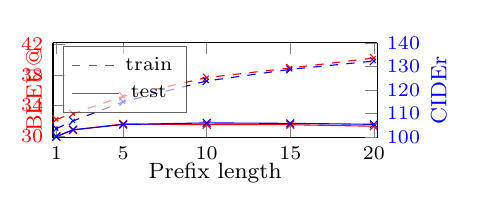
\begin{tikzpicture}
\tikzstyle{every node}=[font=\scriptsize]
\hspace{-.2cm}
\begin{axis}[
    axis y line*=left,
    title={},
    xlabel style={font=\footnotesize, yshift=0.2cm},
    xlabel={Prefix length},
    ylabel style={font=\footnotesize, yshift=-0.5cm, color=red},
    ylabel={BLEU@},
    yticklabel style={color=red},
    xmin=.8, xmax=20.2,
    ymin=29.8, ymax=42.2,
    xtick={1,5,10, 15, 20},
    ytick={30, 34, 38, 42},
    width=.47\textwidth,
    height=.23\textwidth,
]


\addplot[mark=x,red,dashed]
  coordinates{
(1,32.192)(2,32.956)(5,35.1918)(10,37.6397)(15,38.8974)(20,40.1961)
};\label{plot_two}

 \addplot[
    color=red,
    mark=x
    ]
    coordinates {
    (1,30.)(2,30.8)(5,31.6)(10,31.5)(15,31.5)(20,31.3)
    };\label{plot_one}




\end{axis}
\begin{axis}[
axis y line*=right,
  ylabel near ticks,
  yticklabel pos=right,
  axis x line=none,
  yticklabel style={color=blue},
  ylabel style={font=\footnotesize, yshift=0.1cm, color=blue},
  ylabel={CIDEr},
  xmin=.8, xmax=20.2,
  ymin=99.8, ymax=140.2,
  ytick={100, 110, 120, 130, 140},
  width=.47\textwidth,
    height=.23\textwidth,
    legend pos=north west,
    legend style={fill=white, fill opacity=0.6, draw opacity=0.6,text opacity=1},
]







\addlegendimage{dashed,mark options={color=black},color=black}
\addlegendentry{train}
\addlegendimage{mark options={color=black},color=black}
\addlegendentry{test}

\addplot[mark=x,blue,dashed]
  coordinates{
(1,103.678)(2,106.92)(5,115.0527)(10,123.92543)(15,128.85635)(20, 132.393)
};\label{plot_four}
\addplot[mark=x,blue]
  coordinates{
(1,100.2)(2,103.2)(5,105.4)(10,106.1)(15,105.9)(20,105.5)
};\label{plot_three}
\end{axis}
\end{tikzpicture}





 \subcaption{MLP mapping network with fine-tuning of the language model.}
\label{fig:prefix_legnth_mlp}
\end{subfigure}
\begin{subfigure}{\textwidth}
\vspace{3mm}
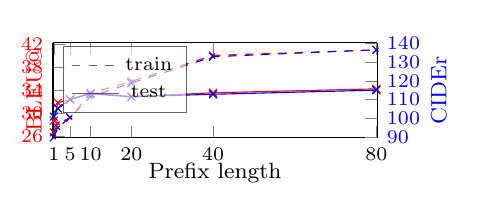
\begin{tikzpicture}
\tikzstyle{every node}=[font=\scriptsize]
\hspace{-.2cm}
\begin{axis}[
    axis y line*=left,
    title={},
    xlabel style={font=\footnotesize, yshift=0.2cm},
    xlabel={Prefix length},
    ylabel style={font=\footnotesize, yshift=-0.5cm, color=red},
    ylabel={BLEU@},
    yticklabel style={color=red},
    xmin=.8, xmax=80.2,
    ymin=25.8, ymax=42.2,
    xtick={1,5,10, 20, 40, 80},
    ytick={26, 30, 34, 38, 42},
    width=.47\textwidth,
    height=.23\textwidth,
]


\addplot[mark=x,red,dashed]
  coordinates{
(1,26.746)(2,28.296)(5,29.275)(10,33.518)(20,35.530)(40,40.015)(80,40.9455)
};\label{plot_two}

 \addplot[
    color=red,
    mark=x
    ]
    coordinates {
    (1,28.746)(2,31.85)(5,32.42)(10,33.53)(20,32.9)(40,33.57)(80,34.244)
    };\label{plot_one}




\end{axis}
\begin{axis}[
axis y line*=right,
  ylabel near ticks,
  yticklabel pos=right,
  axis x line=none,
  yticklabel style={color=blue},
  ylabel style={font=\footnotesize, yshift=0.1cm, color=blue},
  ylabel={CIDEr},
  xmin=.8, xmax=80.2,
  ymin=89.8, ymax=140.2,
  ytick={90, 100, 110, 120, 130, 140},
  width=.47\textwidth,
    height=.23\textwidth,
    legend pos=north west,
    legend style={fill=white, fill opacity=0.6, draw opacity=0.6,text opacity=1},
]







\addlegendimage{dashed,mark options={color=black},color=black}
\addlegendentry{train}
\addlegendimage{mark options={color=black},color=black}
\addlegendentry{test}

\addplot[mark=x,blue,dashed]
  coordinates{
(1,90.0955)(2,95.14)(5,100.6905)(10,111.6430)(20,118.827)(40,132.8)(80,136.500)
};\label{plot_four}

\addplot[mark=x,blue]
  coordinates{
(1,101.04)(2,105.38)(5,110.168)(10,113.08)(20,111.59)(40,112.89)(80,115.069)
};\label{plot_three}
\end{axis}
\end{tikzpicture}






















%
 \subcaption{Transformer mapping network with frozen language model.}
\label{fig:prefix_legnth_transformer}
\end{subfigure}
\caption{Effect of the prefix length on the captioning performance over the COCO-captions dataset. For each prefix length, we report the BLEU@4 (red) and CIDERr (blue) scores over the test and train (dashed line) sets.}
\label{fig:prefix_legnth}
\end{figure} 




\paragraph{Implementation details.}


We used the prefix length of  for the MLP mapping networks, where the MLP contains a single hidden layer. For the transformer mapping network, we set the CLIP embedding to  constants tokens and use  multi-head self-attention layers with  heads each. We train for  epochs using a batch size of . For optimization, we use AdamW \cite{Kingma2015AdamAM} with weight decay fix as introduced by Loshchilov et al.~\cite{loshchilov2017decoupled}, with a learning rate of  and  warm-up steps. For GPT- we employ the implementation of Wolf et al.\cite{wolf-etal-2020-transformers}.





\section{Conclusion}

Overall, our CLIP-based image-captioning method is simple to use, doesn't require any additional annotations, and is faster to train. Even though we propose a simpler model, it demonstrates more merit as the dataset becomes richer and more diverse. We consider our approach as part of a new image captioning paradigm, concentrating on leveraging existing models, while only training a minimal mapping network. This approach essentially learns to adapt existing semantic understanding of the pre-trained models to the style of the target dataset, instead of learning new semantic entities. We believe the utilization of these powerful pre-trained models would gain traction in the near future. Therefore, the understanding of how to harness these components is of great interest. For future work, we plan to incorporate pre-trained models (e.g., CLIP), to other challenging tasks, such as visual question answering or image to D translation, through the utilization of mapping networks. 

